

\begin{abstract} 
This is the abstract, in which we describe why this study is awesome. It's tremendous! Honestly folks, don't trust what the dishonest media say about this study. It is terrific, believe me. 
\end{abstract}  

%\newpage

\section{Introduction}

\epigraph{\textit{
	If you end up with a boring miserable life because you listened to your mom, your dad, your teacher, your priest, or some guy on television telling you how to do your shit, then you deserve it!}}
	{Frank Zappa}

\subsection{Sectioning commands}
\subsubsection[short title for toc]{Even lower-level section with a really, really, long title. Boy, is this a long title!}
\paragraph{This is a paragraph}

\LaTeX will typeset your headlines properly and even count and index them automatically if you use these envirnoments: \verb+\section{}+, \verb+\subsection{}+, \verb+\subsubsection{}+, and \verb+\paragraph{}+. If you want an unnumered section, use the starred version: \verb+\section*{}+



\subsection{Text formatting}
Some \LaTeX-specific formatting tips are provided here. Proper quotation marks are done ``this way'' or \enquote{this way}. 

To add emphasis, words should be in \textit{italics}, not \textbf{bold} or \underline{underlined}. Certainly not \st{strike through}!

A line break requires an empty line between two lines of text in your code. Do not use \verb+\newline+ to force a new paragraph.

There is a difference between three types of dashes: (1) simple dash for composite words such as Latex-specific; (2) double dash for numerical ranges such as 2013--2014; (3) long dashes---I am sure you have seen them before---for included sentences.

There should be a non-separable white space between numbers and their units of measurement: my hat size is 58~cm; not: 58cm. not: 58\newline cm.

\todo[inline]{This is a longer note-to-self kind of text. I describe what I think. Maybe I need to work on this section more. Or delete it? Maybe I just ask my cat what to do with it.}


\subsection{Text shortcuts}
If you use bits of text again and again, make your life easier with
\newline
 \verb+ \newcommand{\blabla}{my little shortcut}+. This turns a long string of text into a tiny little shortcut. I use my \fc a lot, every day a new \fc. Everybody loves the \fc and the \roc! I repeat: \roc, \roc, \roc!




\begin{figure}[t]
	\centering
	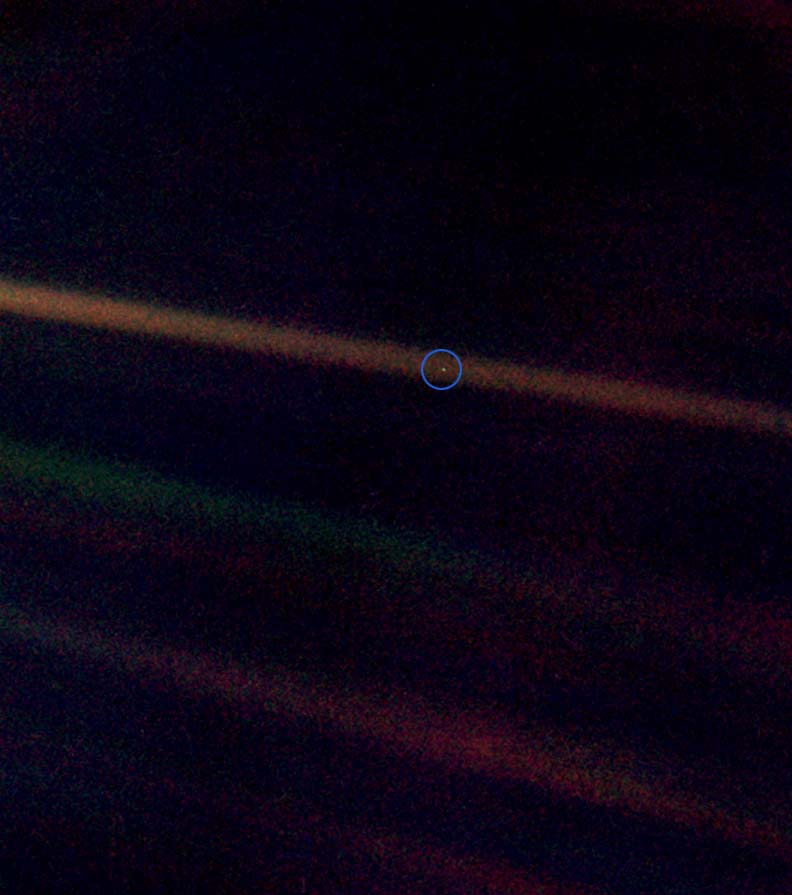
\includegraphics[width=0.25\linewidth]{Figures/PaleBlueDot.jpg}
	\caption{A pale, blue dot, suspended in a sunbeam \citep{NASA}.}
	\label{samplefig}
\end{figure}


\subsection{Environments}

Bullet point environments:
\begin{itemize}
\item In New York;
\item Rio;
\item Tokyo.
\end{itemize}

Enumerated environments:
\begin{enumerate}
\item Stop science funding;
\item Call Wladimir;
\item Build wall.
\end{enumerate}


\subsection{Within-paper references and figures}
\label{withpaperrefs}

You can easily refer to sections within the paper. This is explained in section \ref{withpaperrefs}. You can also refer to figures. The numbering is done fully automatically, see Figure \ref{samplefig} on page \pageref{samplefig}. Note that figures in vector format (.eps; .pdf) are preferred over bitmap formats (.jpg). Figure \ref{pdf_vs_jpg} illustrates why vector formats are better than bitmaps.

We can also use footnotes; little annotations that appear at the bottom of the page\footnotemark.

\footnotetext{This is the footnote text.}


\subsection{Citing literature}


We can refer to papers directly. I greatly admire the study by \cite{ADRIAN1934}. We can also cite papers in parenthesis \citep{ADRIAN1934}. Sometimes, we want to write something additionally into the parentheses \citep[the study by][is also not bad]{Allard2011}. For all details on different ways to cite literature with the natbib package, refer to \url{http://merkel.texture.rocks/Latex/natbib.php}. 

We can also typeset quotes nicely:

\begin{displayquote}
The aggregate of all our joys and sufferings, thousands of confident religions, ideologies and economic doctrines, every hunter and forager, every hero and coward, every creator and destroyer of civilizations, every king and peasant, every young couple in love, every hopeful child, every mother and father, every inventor and explorer, every teacher of morals, every corrupt politician, every superstar, every supreme leader, every saint and sinner in the history of our species, lived there---on a mote of dust, suspended in a sunbeam \citep[][S. 6--7; see Figure \ref{samplefig}]{Sagan1994}.
\end{displayquote}


\todo[]{Anything else I should mention here?}




\begin{figure}[t]
	\centering
	
	\begin{subfigure}[t]{0.45\textwidth}
		\centering
		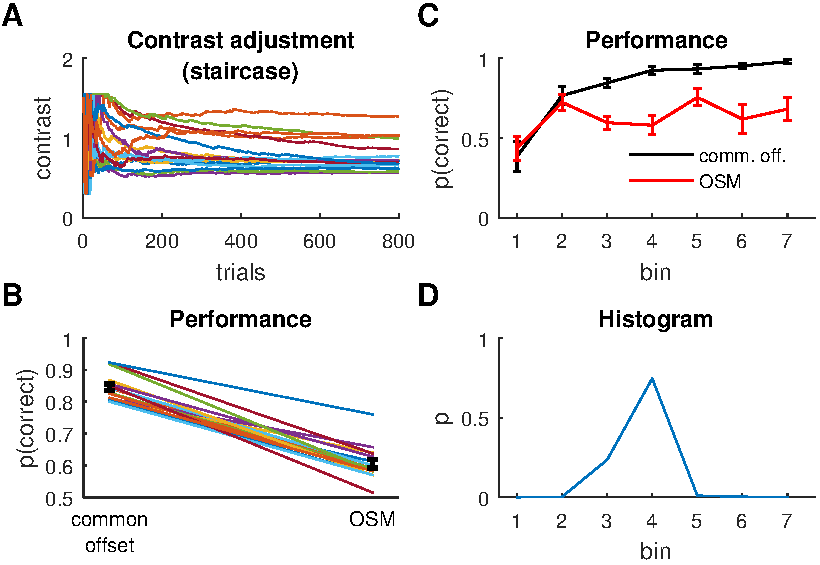
\includegraphics[width=\linewidth]{Figures/Resultspdf} 
	\end{subfigure}		
	\hfill % If you want to place the figures side by side there should be no empty line between subfigures.		
	\begin{subfigure}[t]{0.45\textwidth}
		\centering
		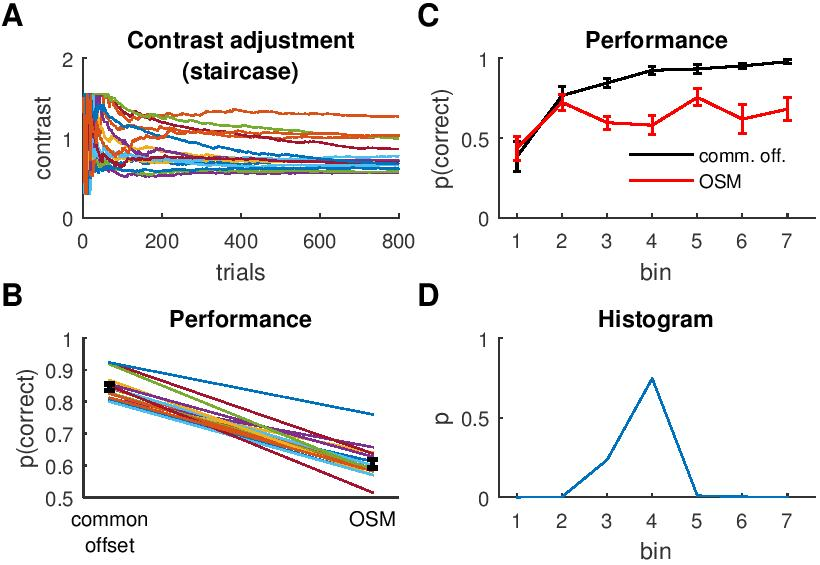
\includegraphics[width=\linewidth]{Figures/Resultsjpg} 
	\end{subfigure}
	
	
	\caption{Comparison of vector format and bitmap format. Left: figure built from a *.pdf file. The separate lines are easy to see, can be zoomed in and text is searcheable in the pdf output. Right: figure built from *.jpg. Doesn't look so good.}
	\label{pdf_vs_jpg}
\end{figure}
